\section{Exercise 4 - Binary Tree Algorithms for \texttt{MPI\_Bcast} and \texttt{MPI\_Reduce}}
Text for Ex4.
\begin{figure}[h]
    \begin{center}
        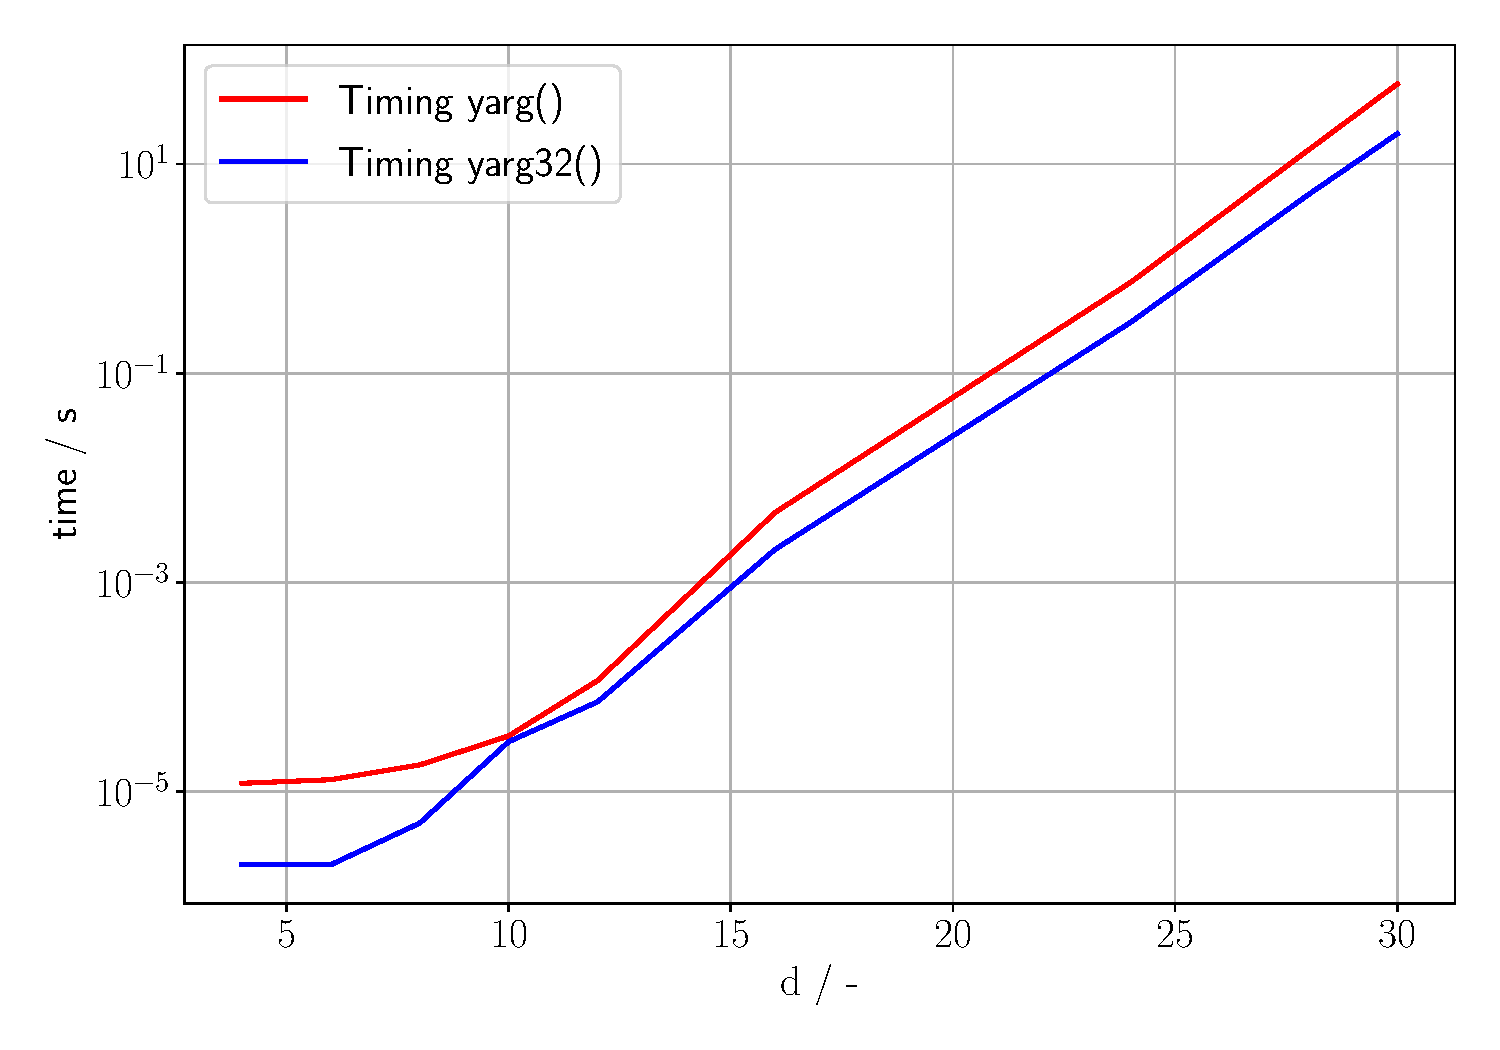
\includegraphics[width= 0.88\linewidth]{figures/task_5_plot.pdf} 
        \label{ref_plot_task_5}
        \caption{Benchmark both algorithms - \texttt{yarg32()} is faster than \texttt{yarg()} for all feasible values of $d$}
    \end{center}
\end{figure}
\pagebreak

\section{Exercise 5 - Integrated, Improved Binary Tree Algorithm}
Text for Ex5.
\begin{equation}
    \begin{aligned}
        \sum_{i=0}^d k^i &= \sum_{i=0}^d k^i \\
        \sum_{i=0}^d k^i - k \sum_{i=0}^d k^i &= \sum_{i=0}^d k^i - k \sum_{i=0}^d k^i \\
        \sum_{i=0}^d k^i - k \sum_{i=0}^d k^i &= \sum_{i=0}^d k^i - \sum_{i=1}^{d+1} k^i \\
        \sum_{i=0}^d k^i \, (1-k) &= 1 - k^{d+1}\\
        \sum_{i=0}^d k^i   &=  \frac{k^{d+1} - 1}{k-1}
        \label{closedForm_Ex1.1}
    \end{aligned}
    \end{equation}
\pagebreak

\section{Exercise 6 - Improvement with Sibling Leave Communication (BONUS)}
Text for Ex6.
\pagebreak


\section{Exercise 7 - Implemenetation and Benchmarking of Improved Version (BONUS)}
Text for Ex7.
\pagebreak